\chapter{Lecture 8}

This lecture is about \texttt{Classification And Regression Trees
Discussion of Case 1 and case competition} where chapter \texttt{ESL Chapter 9.2} should be looked upon.


Tree-based methods partition the feature space into a set of rectangles, and then fit a simple model.



\section{Regression Trees}

To evaluate the goodness of a new split, we can now simply compute the average sum-of-squares error between the observed $y_i$'s and the mean value $y(v_2)$. This can be done by simply introducing a new impurity measure seen more below

%\[
%    I(v) = \frac{1}{N(v)} \sum_{i \in v} (y_i - y(v))^2 \quad \text{ where } \quad y(v) = \frac{1}{N(v)} \sum_{i \in v} y_i
%\]

Our data consists of $p$ inputs and a response, for each of $N$ observations: that is, $(x_i, y_i)$ for $i=1, 2, ..., N$ with $x_i = (x_{i1}, x_{i2},...,x_{ip}$. The algorithm
needs to automatically decide on the splitting variables and split points, and also what topology (shape) the tree should have. Suppose first that we have a partition into $M$ regions $R_1, R_2, ..., R_M$ and we model the response as a constant $c_m$ in each region

\[
    f(x) = \sum_{m=1}^{M} c_m I(x \in R_m)
\]

If we adopt as our criterion minimization of the sum of squares

\[
     \sum_{i \in v} (y_i - y(v))^2
\]

then the best $\hat{c}_m$ is just the average of $y_i$ in region $R_m$

\[
    \hat{c}_m = ave(y_i | x_i \in R_m)
\]
More from \cite[p.~307]{friedman2016elements}
How large should we grow the tree? Clearly a very large tree might overfit the data, while a small tree might not capture the important structure.

Tree size is a tuning parameter governing the model’s complexity, and the
optimal tree size should be adaptively chosen from the data. One approach
would be to split tree nodes only if the decrease in sum-of-squares due to the
split exceeds some threshold. This strategy is too short-sighted, however,
since a seemingly worthless split might lead to a very good split below it.

From lecture \cite[p.~31]{lecture8}, then the way to find the right sized tree, is to grow the tree really large and then decide which splits were unnecessary and remove these.

This is called \textbf{pruning} the tree. Pruning a node amounts to removing its sub-tree, thereby making a terminal node

From \cite[p.~308]{friedman2016elements} then the preferred strategy is to grow a large tree $T_0$ stopping the splitting process only when some minimum node size is reached. Then this large tree is pruned using \textit{cost-complexity pruning} , which we now describe.

We define a subtree $T \subset T_0$ to be any tree that can be obtained by pruning $T_0$, that is, collapsing any number of its internal nodes. We index terminal nodes by $m$ with node $m$ representing region $R_m$. Let $|T|$ denote the number of terminal nodes in $T$. Letting

\[
    N_m = \# \{x_i \in R_m\}
\]

\[
    \hat{c}_m = \frac{1}{N_m} \sum_{x_i \in R_m} y_i
\]

To evaluate the goodness of a new split, we can now simply compute the average sum-of-squares error between the observed $y_i$'s and the mean value $\hat{c}_m$. This can be done by simply introducing a new impurity measure:

\[
    Q_m (T) = \frac{1}{N_m} \sum_{x_i \in R_m}  (y_i - \hat{c}_m)^2
\]

we define the cost complexity criterion

\[
    C_\alpha (T) = \sum_{m=1}^{T} N_m Q_m (T) + \alpha |T|
\]

The idea is to find, for each $\alpha$, the subtree $T_\alpha \subseteq T_0$ to minimize $C_\alpha (T)$.
The tuning parameter $\alpha \geq 0$ governs the tradeoff between tree size and its goodness of the fit to the data.  \cite[p.~308]{friedman2016elements}

\section{Classification Trees}

For regression we used sum of squares error node impurity measure, but this is not suitable for classification. In a node $m$, representing a region $R_m$, with $N_m$ observations, let

\[
    \hat{p}_{mk} = \frac{1}{N_m} \sum_{x_i \in R_m} I ( y_i = k)
\]

the proportion of class $k$ observations in node $m$.

We classify observations in the node to class

\[
    K = \arg \max\limits_k \hat{p}_k
\]

Then different measures of node impurity include the following\\

The misclassification error

\[
    Q_m(T) = \frac{1}{N_m} \sum_{i \in R_m} I(y_i \neq k(m)) = 1 - \hat{p}_{mk(m)}
\]

The Gini index:

\[
    Q_m(T) = \sum_{k \neq k'} \hat{p}_{mk} \hat{p}_{mk'} = \sum_{k=1}^{K}  \hat{p}_{mk} (1 -  \hat{p}_{mk})
\]

The Cross Entropy or deviance:

\[
    Q_m (T) = - \sum_{k=1}^{K}  \hat{p}_{mk} \log (  \hat{p}_{mk} )
\]

\begin{figure}[H]
  \centering
  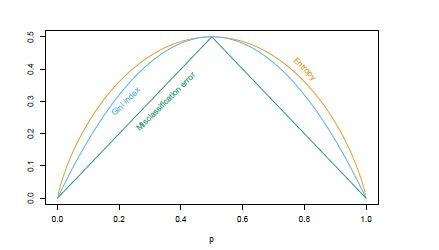
\includegraphics[width=0.9\textwidth]{treeclassificationthreeerrors}
  \caption{ode impurity measures for two-class classification, as a function of the proportion p in class 2. Cross-entropy has been scaled to pass through (0.5, 0.5).}\label{fig:treeclassificationthreeerrors}
\end{figure}

The node impurity is weighted with the number of observations in
each node.
The split decision is based on the split that minimizes,

\[
    N_{\text{left}}Q_{\text{left}} + N_{\text{right}}Q_{\text{right}}
\]

where, $N$ is the number of observations in left or right node and $Q$ is node impurity for left or right node. Lower is better.

Entropy and Gini index are
better measures for
growing tree because they
are more sensitive to node
probabilities. Use Gini index as split criterion when building the tree and Use missclassification rate as criterion when deciding which
node to prune from lecture \cite[p.~54-55]{lecture8}

\subsection{Missing data}

We can always, delete the observation or replace with mean or median.

For trees we can introduce an extra category "missing" - if it is a categorical variable or we can use a surrogate variable. In each branch, have a list of alternative variables and split points - as a backup.

From lecture \cite[p.~3]{lecture9} we know that:

\begin{itemize}
  \item Advantage:
  \begin{itemize}
    \item Interpretability, tree defines a set of rules which are easy to follow.
    \item Handles missing data.
    \item Can take both continuous and categorical variables as input.
  \end{itemize}
  \item Drawback:
  \begin{itemize}
    \item Deep trees have high variance and low bias.
    \item Small trees have low variance and high bias.
    \item New data might completely change the shape of the tree.
  \end{itemize}
\end{itemize}
